
\chapter{Writing \LaTeX}

This is the start of a chapter and gives some introduction before its first section.  This chapter describes basic \LaTeX{} you need to know.

%%%%%%%%%%%%%%%%%%%%%%%%%%%%%%%%%%%%%%%%%%%%%%%%%%%%%%%%%%%%%%%%%%%%
\section{Sectioning}
\label{sec:sectioning}

The following sectioning macros are available, ordered in descending
importance:

\begin{verbatim}
\chapter{A Chapter}
\section{A Section}
\subsection{A Sub Section}
\subsubsection{A Sub Sub Section}
\subsubsubsection{A Sub Sub Sub Section}
\end{verbatim}

Three-sub's is all you get.  
Consult with the technical editors if you feel finer grained
sectioning is required.
Starting from \verb|\subsection|, this produces the following:

\subsection{A Sub Section}
\subsubsection{A Sub Sub Section}
\subsubsubsection{A Sub Sub Sub Section}

Just after defining a chapter and any significant section a
\verb|\label| should be added so it can be referenced.
A label can be added later for a `'less significant'' section that
turns out to need one. You can label them all. 

For example:

\begin{verbatim}
\chapter{A Chapter}
\label{ch:a-chapter}

\section{A Section}
\label{sec:a-section}

\subsection{A Sub Section}
\label{subsec:a-subsection}
\end{verbatim}

See Section~\ref{sec:refs} for how to reference labeled sections.

\FloatBarrier
%%%%%%%%%%%%%%%%%%%%%%%%%%%%%%%%%%%%%%%%%%%%%%%%%%%%%%%%%%%%%%%%%%%%
\section{Figures}
\label{sec:figures}

See Section~\ref{sec:figure-format} for guidelines on the graphics files themselves.
Instead of using the usual \texttt{figure} environment a custom \texttt{cdrfigure}
environment is used in order to provide for a consistent presentation.
The environment is called with one optional and two required
arguments:

\begin{enumerate}
\item An initial, optional short caption for the List Of Figures, in square brackets.
\item A label for referencing (it will have \texttt{fig:} prepended). Curly brackets.
\item The full caption. Curly brackets, again.
\end{enumerate}

This is followed by including the graphic file.

\begin{cdrfigure}[Short ToF caption]{aerial}{An aerial photograph of Fermilab
    showing Wilson Hall and surrounding accelerator rings (Fermilab
    Visual Media Services)}
  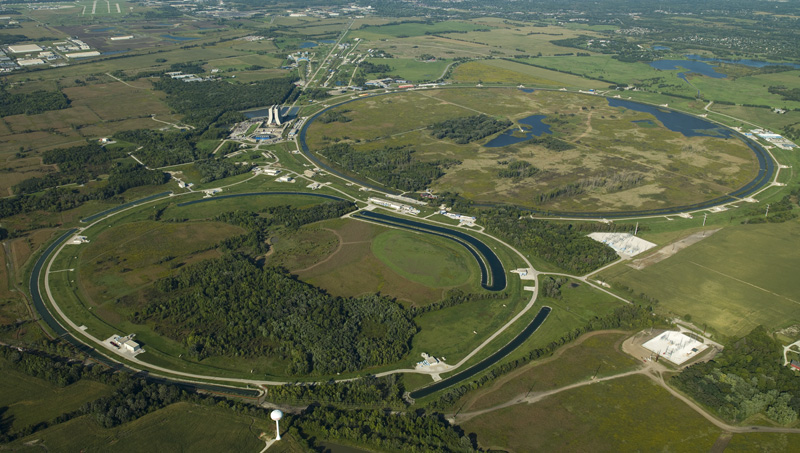
\includegraphics[width=0.8\textwidth]{fermilab-aerial.jpg}
\end{cdrfigure}


When the figure contains a graphic,  usually \texttt{includegraphics} is used.
The filename is assumed relative to a volume-specific \texttt{graphicspath} as
described in Section~\ref{sec:files} and as such one typically should
\textbf{not} specify any directory parts in its name.
The file's extension may be omitted.
An example can be seen in Figure~\ref{fig:aerial}, which is created
with the following \LaTeX shown in Figure~\ref{fig:aerial-latex}

\begin{cdrfigure}{aerial-latex}{\LaTeX{} showing how to do include a figure.}
\begin{verbatim}
\begin{cdrfigure}[Short ToF caption.]{aerial}{An aerial photograph of Fermilab
    showing Wilson Hall and surrounding accelerator rings (Fermilab
    Visual Media Services)}
  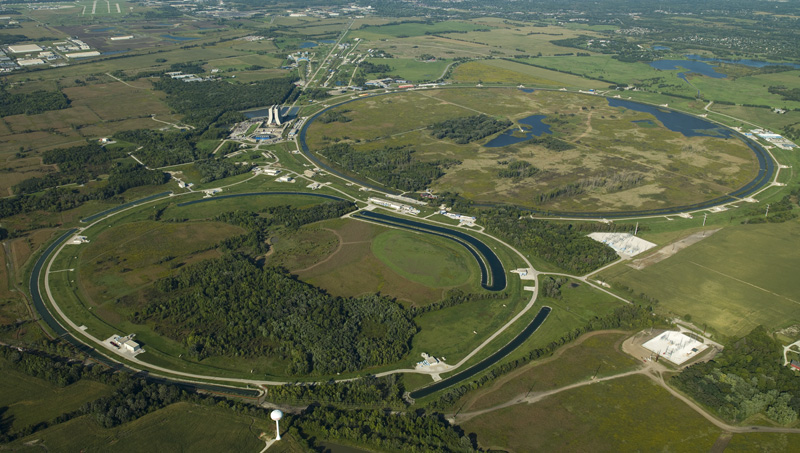
\includegraphics[width=0.8\textwidth]{fermilab-aerial.jpg}
\end{cdrfigure}
\end{verbatim}
\end{cdrfigure}

\FloatBarrier
%%%%%%%%%%%%%%%%%%%%%%%%%%%%%%%%%%%%%%%%%%%%%%%%%%%%%%%%%%%%%%%%%%%%
\section{Tables}
\label{sec:tables}

Like figures, we use a special environment, \texttt{cdrtable} for
tables to achieve a degree of consistency.
This is instead of the usual double \texttt{table} + \texttt{tabular} environments.
The \texttt{cdrtable} environment takes one optional and three
required arguments:

\begin{enumerate}
\item An initial, optional short caption for the List of Tables. Square brackets.
\item The tabular column specification. Curly brackets for the last three.
\item A label for referencing (it will have \texttt{tab:} appended)
\item The full caption.
\end{enumerate}

Inside the actual contents of the table you are required to provide a
initial row containing the headings for the table's rows followed by a
\texttt{toprowrule} macro.
Following every regular row (except the last) you should include a
\texttt{colline} macro.
Both of these take the place of the usual \texttt{hline}.

\begin{cdrtable}[The LoT caption]{cc}{example}
{This is an example table. We will use better colors, don't worry.}
  Rows & Counts \\ \toprowrule
  Row 1 & First \\ \colhline
  Row 2 & Second \\ \colhline
  Row 3 & Third \\ 
\end{cdrtable}

\noindent Table~\ref{tab:example} is thus made like (arguments can span lines):

\begin{verbatim}
\begin{cdrtable}[The LoT caption]{cc}{example}
{This is an example table. We will use better colors, don't worry.}
  Rows & Counts \\ \toprowrule
  Row 1 & First \\ \colhline
  Row 2 & Second \\ \colhline
  Row 3 & Third \\ 
\end{cdrtable}
\end{verbatim}

Table~\ref{tab:pdecay} shows a more complex example.
See the source for how it is written.
Note that special column specifications are used.

\begin{cdrtable}[Efficiencies and background rates for nucleon decay
  modes]{$L^c^c^c^c}{pdecay}{Efficiencies and background rates for
    nucleon decay channels of interest for a large underground LArTPC,
    and comparison with water Cherenkov detector capabilities} %$
  Decay Mode & \multicolumn{2}{^c}{Water Cherenkov} & 
\multicolumn{2}{^c}{Liquid Argon TPC} \\
\rowtitlestyle
& Efficiency & Background & Efficiency & Background \\ \toprowrule
$p \rightarrow K^+ \overline{\nu}$ & 19\% & 4 & 97\% & 1 \\ \colhline
$p \rightarrow K^0 \mu^+$ & 10\% & 8 & 47\% & $<2 $ \\ \colhline
$p \rightarrow K^+ \mu^- \pi^+$ & & & 97\% & 1 \\ \colhline
$n \rightarrow K^+ e^- $ & 10\% & 3 & 96\% & $<2$ \\ \colhline
$n \rightarrow e^+\pi^-$ & 19\% & 2 & 44\% & 0.8 \\
\end{cdrtable}

\FloatBarrier
%%%%%%%%%%%%%%%%%%%%%%%%%%%%%%%%%%%%%%%%%%%%%%%%%%%%%%%%%%%%%%%%%%%%
\section{Referencing and Citations}
\label{sec:refs}

Note: if you see a grey label blox containing \texttt{sec:refs}
between this paragraph and the section heading (or in general
elsewhere in chapters, sections, figures, etc), it means this document
was built in draft mode.  
These artifacts show up to help you know what label was used to
reference each particular thing.


\subsection{Intra-document References}

Assume that any chapter, section or important sub-, subsub-, section
or within any figure or table environment may need to be referenced
elsewhere in the text. As described in Section~\ref{sec:sectioning},
define a label (\verb|\label{...}| for these items.
Use the defined label in a \verb|\ref{...}| in order to make reference
to the chapter, section, figure, etc.
For example:

\begin{verbatim}
\chapter{Some Chapter}
\label{ch:some-chapter}

\subsection{Some Sub Section}
\label{subsec:some-sub-section}

...

As described in Chapter~\ref{ch:some-chapter} ...

As shown in Figure~\ref{fig:fermilab-aerial} ...
\end{verbatim}

When you reference a chapter, section, subsection, figure, table,
etc., capitalize the word ``Chapter'' or whatever it is, e.g., ``as
shown in Section~\ref{sec:plots}.''
Use the word ``Section'' even if it's a subsection or subsubsection,
and use the tilde sign to keep the number on the same line as the word
that precedes it.

Examples for figures and tables have been given above.  Here I
reference this section:~\ref{sec:refs}.  


\subsection{Citations}

Referencing citations is done like \verb|\cite{strunk}| which gives \cite{strunk}.
The key \texttt{strunk} matches an entry in the \texttt{citedb.bib}
file in the top-level directory.


The \texttt{citedb.bib} file is in BitTex format.
This is \textbf{not} \LaTeX{} format and in particular does not
indicate comments via \texttt{\%} characters.
The content and order of entries in this file is not reflected in the
generated Bibliography.
However, manual care must be taken to avoid duplication.
Before adding any entry to \texttt{citedb.bib} read/search through it
to ascertain that the entry you wish to add is not already there.






